\documentclass[11pt,a4paper]{article}
\usepackage[margin=2.5cm]{geometry}
\usepackage{amsmath,amssymb,amsthm}
\usepackage{graphicx,booktabs,microtype}
\usepackage{xcolor}
\usepackage[colorlinks=true,linkcolor=blue!50!black,citecolor=blue!50!black,urlcolor=blue!50!black]{hyperref}

\newtheorem{proposition}{Proposition}
\newcommand{\R}{\mathbb{R}}
\newcommand{\tr}{^{\mathsf T}}

\title{A coarse-space preconditioner for multiple-shooting Newton--Krylov:\\
GMRES iterations independent of the period}
\author{Notes for NKSearch.jl, branch \texttt{coarse-precond}}
\date{October 2026}

\begin{document}
\maketitle

\begin{abstract}
In a multiple-shooting Newton--Krylov search with segments of fixed length $\tau$, the number of GMRES iterations per Newton step grows with the period $T$: faster than linearly with the regular row ordering, and linearly with the Ashtari ordering used by NKSearch. With the Ashtari ordering the Newton operator is $-I$ plus a cyclic block subdiagonal of segment tangent maps, and its spectrum consists of one circle of radius $e^{\lambda\tau}$ around $-1$ for every Floquet exponent $\lambda$. The linear growth comes only from the few circles of the unstable and neutral directions, which surround the origin. We remove them with a coarse space spanned, at every shooting point, by the leading covariant subspace of the tangent dynamics. The resulting right preconditioner is $-I$ outside the coarse space and an exact Galerkin solve on it; the coarse problem is small, cyclic and block-bidiagonal, and must be factorised by QR. For Kuramoto--Sivashinsky the number of GMRES iterations becomes 4 (rtol $10^{-6}$) at every period from 16 to 2048, as predicted by the first excluded Lyapunov exponent, and full Newton searches on orbits with periods 53 to 425 take 2--3 GMRES iterations per step. The total work of a search becomes proportional to $T$ instead of $T^2$, including the cost of building the subspaces. The method is the multiple-shooting counterpart of the Newton--Picard method of Lust et al., used as a Krylov preconditioner.
\end{abstract}

\tableofcontents

%======================================================================
\section{The multiple-shooting Newton system}
%======================================================================

We look for a periodic orbit of $\dot x = f(x)$, $x \in \R^n$, with $N$ shooting points $x_1,\dots,x_N$ and period $T$. Let $\varphi_t$ be the flow and $\tau = T/N$ the segment length. The equations are
\begin{equation}
F_i(x, T) = \varphi_{\tau}(x_i) - x_{i+1} = 0, \qquad i = 1,\dots,N, \qquad x_{N+1} \equiv x_1,
\end{equation}
(for a relative periodic orbit the last segment is followed by the shift $S(\cdot, s)$, and $s$ is a further unknown). One Newton step solves for $(\delta x_1,\dots,\delta x_N, \delta T)$
\begin{equation}
M_i\,\delta x_i - \delta x_{i+1} + \frac{1}{N}\,\dot x_i^{T}\,\delta T = -F_i, \qquad
f(x_1)\tr \delta x_1 = 0,
\label{eq:newton}
\end{equation}
where $M_i = \partial\varphi_\tau/\partial x\,(x_i)$ is the tangent map of segment $i$ and $\dot x_i^T$ the derivative of its end point with respect to the period (computed by finite differences in NKSearch). The last row is the phase condition. In NKSearch the action of the operator costs one tangent integration per segment, done in parallel over segments.

\paragraph{Row orderings.} With the \emph{regular} ordering, row block $i$ holds equation $i$: the diagonal blocks are $M_i$ and the superdiagonal blocks $-I$. With the \emph{Ashtari} ordering (the NKSearch default), equation $i$ is placed in row block $i+1$. The diagonal blocks become $-I$ and the tangent maps move to the subdiagonal:
\begin{equation}
A = -I + C + (\text{period column, phase row}), \qquad
C = \begin{pmatrix}
0 & & & M_N\\
M_1 & 0 & & \\
 & \ddots & \ddots & \\
 & & M_{N-1} & 0
\end{pmatrix}.
\label{eq:ashtari}
\end{equation}
The reordering is a row permutation: it does not change the solution, but it changes the spectrum completely, and GMRES only sees the spectrum (and the non-normality).

%======================================================================
\section{Why GMRES needs $O(N)$ iterations}
%======================================================================

\begin{proposition}\label{prop:spectrum}
Let $\Phi = M_N \cdots M_1$ be the monodromy matrix (at $x_1$) with eigenvalues $\mu_1,\dots,\mu_n$ (Floquet multipliers, all nonzero). The eigenvalues of $C$ in \eqref{eq:ashtari} are the $nN$ numbers $\sigma$ with $\sigma^N = \mu_j$, i.e.\ $\sigma = \mu_j^{1/N} e^{2\pi i m/N}$, $m = 0,\dots,N-1$. Hence the eigenvalues of $-I + C$ are
\[
-1 + |\mu_j|^{1/N} e^{i(\arg\mu_j + 2\pi m)/N}:
\]
for every multiplier, $N$ points on the circle of centre $-1$ and radius $|\mu_j|^{1/N} = e^{\lambda_j \tau}$, where $\lambda_j = \log|\mu_j|/T$ is the Floquet exponent.
\end{proposition}

\begin{proof}
$C^N$ is block diagonal with blocks $M_{i-1}\cdots M_1 M_N \cdots M_i$, all similar to $\Phi$. If $Cv = \sigma v$ then $C^N v = \sigma^N v$, so $\sigma^N$ is a multiplier. Conversely, if $\Phi u = \mu u$ and $\sigma^N = \mu$, the vector with blocks $v_1 = u$, $v_{i+1} = \sigma^{-1} M_i v_i$ satisfies $Cv = \sigma v$ (the last block closes because $\sigma^{-N}\Phi u = u$).
\end{proof}

The radius $e^{\lambda_j\tau}$ depends on the segment length only, not on $T$: making the orbit longer at fixed $\tau$ adds points on the same circles. Two cases follow.

\begin{itemize}
\item \textbf{Contracting directions}, $\lambda_j < 0$. The circle lies inside the disc $|z+1| < 1$ and stays away from the origin. GMRES reduces these components by roughly $e^{\lambda_j\tau}$ per iteration, whatever $N$.
\item \textbf{Unstable and neutral directions}, $\lambda_j \ge 0$. The circle surrounds or touches the origin. The GMRES residual polynomial $p$ has $p(0) = 1$ and must be small at $N$ points that surround $0$; for points equally spaced on such a circle this needs degree $\approx N$. The extreme case is the cyclic shift ($M_i = I$), for which GMRES makes no progress for $N-1$ iterations. Physically, each matrix-vector product moves information by one segment, and the unstable components must travel once around the whole orbit.
\end{itemize}

So with the Ashtari ordering the iteration count is $O(N) = O(T/\tau)$, and the work of a Newton step (iterations $\times$ $N$ segment integrations) is $O(T^2)$. Figure~\ref{fig:spectrum} shows the spectra for KS: the Ashtari spectrum is a set of concentric circles around $-1$, and the outermost ones pass through the origin. With the regular ordering the eigenvalues fill a region around the origin, and GMRES does worse.

\begin{figure}[t]
\centering
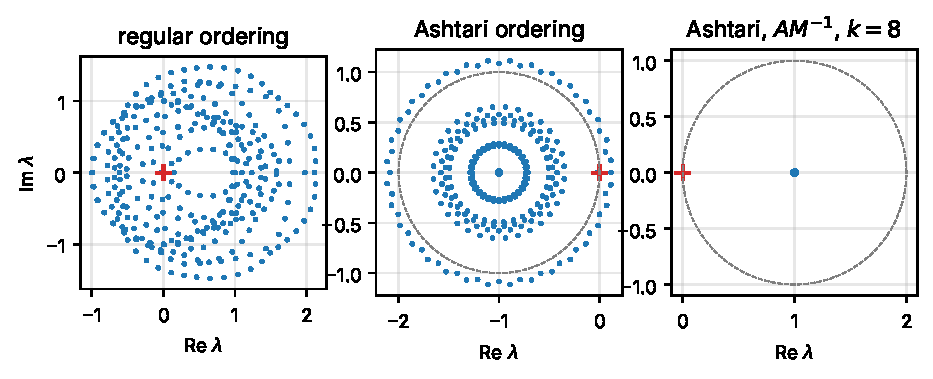
\includegraphics[width=\textwidth]{figs/spectrum.pdf}
\caption{Eigenvalues of the NKSearch Newton operator for KS ($L = 39$, odd subspace, 32 modes) along a chaotic trajectory, $N = 32$ segments of length $\tau = 2$, assembled column by column from the code (\texttt{spectrum.jl}). Left: regular ordering. Middle: Ashtari ordering; the dashed circle has centre $-1$ and radius 1. Right: preconditioned operator $AM^{-1}$ with $k = 8$; all 1025 eigenvalues lie within $0.014$ of $1$ (dashed: circle of radius 1 around 1). The red cross marks the origin.}
\label{fig:spectrum}
\end{figure}

%======================================================================
\section{The coarse space and the preconditioner}
%======================================================================

\subsection{Invariant covariant subspaces}

Order the multipliers by modulus and assume a gap, $|\mu_k| > |\mu_{k+1}|$. Let $U_1$ be the invariant subspace of $\Phi$ for $\mu_1,\dots,\mu_k$, and $U_{i+1} = M_i U_i$. These are the leading covariant (Floquet) subspaces at the shooting points; they satisfy $M_i U_i = U_{i+1}$ exactly, including $M_N U_N = U_1$. Therefore the space
\[
\mathcal W = U_1 \oplus \cdots \oplus U_N \subset \R^{nN}
\]
is invariant under $C$, and so under $-I + C$: the Newton operator maps $\mathcal W$ into itself. It carries exactly the eigenvalues of Proposition~\ref{prop:spectrum} with $j \le k$.

Let $V_i \in \R^{n\times k}$ be orthonormal bases of $U_i$, and $W = \mathrm{blockdiag}(V_1,\dots,V_N, I_{N_s})$, where the last block keeps the $N_s$ scalar unknowns (period, and shift if present) in the coarse space. $W$ has orthonormal columns. The coarse matrix is the Galerkin projection $E = W\tr A W$, of size $Nk + N_s$.

\subsection{The preconditioner}

We use the right preconditioner
\begin{equation}
M^{-1} = -(I - WW\tr) + W E^{-1} W\tr, \qquad M = -(I - WW\tr) + W E W\tr .
\label{eq:precond}
\end{equation}
It is the inverse of the Ashtari diagonal ($-I$) outside the coarse space, and an exact solve on it. GMRES is applied to $AM^{-1}y = b$, then $x = M^{-1}y$; right preconditioning leaves the residual unchanged. Both $M$ and $M^{-1}$ are cheap, which lets us map a warm start $x_0$ to $y_0 = Mx_0$ exactly.

\begin{proposition}
Ignore the period column and phase row, and assume $\mathcal W$ is exactly invariant. In the splitting $\R^{nN} = \mathcal W \oplus \mathcal W^\perp$, $A$ is block upper triangular, and $AM^{-1}$ has the eigenvalue $1$ on $\mathcal W$ and, on the complement, the eigenvalues $1 - \sigma$ with $\sigma^N = \mu_j$, $j > k$: circles of radius $e^{\lambda_j\tau}$ around $1$.
\end{proposition}

\begin{proof}
$A\mathcal W \subset \mathcal W$ makes $A = \begin{pmatrix} E & A_{12}\\ 0 & A_{22}\end{pmatrix}$, so the eigenvalues of $A_{22}$ are those of $A$ not carried by $\mathcal W$. In the same splitting $M^{-1} = \mathrm{diag}(E^{-1}, -I)$, so $AM^{-1} = \begin{pmatrix} I & -A_{12} \\ 0 & -A_{22}\end{pmatrix}$.
\end{proof}

Hence GMRES converges at a rate set by the first excluded exponent,
\begin{equation}
m \approx \frac{\log \mathrm{rtol}}{\lambda_{k+1}\tau},
\label{eq:predict}
\end{equation}
independently of $N$ and $T$ (up to non-normality, and to the bordering, which adds a rank-$N_s$ coupling that GMRES absorbs in a few iterations). Section~\ref{sec:results} checks \eqref{eq:predict} quantitatively.

\subsection{Building the subspaces}

The bases are obtained by subspace iteration around the orbit, all segments in parallel:
\[
P_i = M_i V_i \ (\text{$k$ tangent integrations per segment}), \qquad V_{i+1} \leftarrow \mathrm{orth}(P_i)
\]
(the last segment includes the shift). Each sweep advances every basis by one segment. The leading covariant subspace at a point depends only on the recent past of the trajectory, with errors decaying roughly as $e^{(\lambda_{k+1} - \lambda_k)\tau}$ per sweep, so the number of sweeps needed does not grow with $N$. In NKSearch:
\begin{itemize}
\item at the first Newton step, $V_i$ are random and \texttt{coarse\_sweeps} sweeps are done;
\item at every later step, the images $P_i$ of the previous step (computed at the previous orbit) are used as a warm start, $V_{i+1} \leftarrow \mathrm{orth}(P_i)$, without new integrations;
\item then one more round $P_i = M_iV_i$ gives the blocks of $E$:
\[
E_{i+1,i} = V_{i+1}\tr P_i, \quad E_{i+1,i+1} = -I_k, \quad E_{i+1,T} = V_{i+1}\tr \dot x^T_i/N, \quad E_{\text{phase},1} = f(x_1)\tr V_1 .
\]
\end{itemize}
So in steady state a Newton step costs $k$ tangent integrations per segment for the coarse space.

\paragraph{Choosing $k$.} $k$ must exceed the number of unstable and neutral directions, and it is best placed at a spectral gap. If $\lambda_k - \lambda_{k+1}$ is small, the subspace converges slowly; GMRES still converges, but with an iteration count that again grows with $N$ (Table~\ref{tab:sweeps}).

\subsection{The coarse solve must use QR}

$E$ is sparse, cyclic and block-bidiagonal, with $k\times k$ blocks, plus the bordering. A direct factorisation costs $O(Nk^3)$ operations. Gaussian elimination with partial pivoting is unstable on matrices with this structure~\cite{wright1993}: the growth around the cycle is $e^{\lambda_1 T}$, and once it exceeds $1/\varepsilon$ the LU solve is wrong. We observed exactly this: at $T = 1024$ (growth $e^{41}$) GMRES reported convergence while the true residual $\|Ax - b\|/\|b\|$ was $10^3$--$10^4$. A sparse QR factorisation (SuiteSparse SPQR) is backward stable and fixes it; all results below use QR.

%======================================================================
\section{Cost}
%======================================================================

Count the cost in segment tangent integrations $c$ (each re-integrates the base flow for one segment, as in NKSearch). Let $m_0$ and $m_k$ be the GMRES iterations without and with the coarse space, $n_N$ the number of Newton steps and $s$ = \texttt{coarse\_sweeps}.

\begin{center}
\begin{tabular}{lll}
\toprule
 & work per Newton step & wall time on $N$ workers \\
\midrule
no preconditioner & $m_0 N c$, \ $m_0 \propto N$: \ $\propto T^2$ & $m_0 c \propto T$\\
coarse, steady state & $(m_k + k) N c$: \ $\propto T$ & $(m_k + k)c$: constant\\
coarse, first step (extra) & $s k N c$ & $s k c$\\
\bottomrule
\end{tabular}
\end{center}

A whole search costs $N[\,n_N(m_k + k) + sk\,]c$ with the coarse space against $N n_N m_0 c$ without. The other costs are small:
\begin{itemize}
\item \emph{Coarse QR}: $O(Nk^3)$ flops per Newton step. For a PDE this is negligible next to one tangent integration.
\item \emph{Applying $M^{-1}$}: $k$ inner products and $k$ axpys per segment.
\item \emph{Memory}: $V$ and $P$ hold $2Nk$ states. This is the main overhead for large states: for example $N = 200$, $k = 30$ and $256^2$ grids need about 6\,GB. It is partly offset by the Krylov basis, which shrinks from $m_0 N$ to $m_k N$ states. $P$ could be dropped and recomputed at the price of $k$ integrations per step.
\end{itemize}
On a GPU the $k$ images of a segment can be integrated as one batch (one base flow, $k$ tangent vectors), which makes the coarse space cheaper than $k$ separate integrations.

%======================================================================
\section{Results for Kuramoto--Sivashinsky}
\label{sec:results}
%======================================================================

\paragraph{Set-up.} $u_t = -uu_x - u_{xx} - u_{xxxx}$ on $L = 39$ in the odd subspace, as in the ReSolver notes: 32 sine coefficients, the advection term evaluated on 128 points (no aliasing), IMEX CB3R2R3e with $\Delta t = 0.025$ from Flows.jl, and the exact coupled tangent (\texttt{ks.jl}). Segments have length $\tau \approx 2$. The first Lyapunov exponents along the attractor are

\begin{center}
\small
\begin{tabular}{l*{10}{r}}
\toprule
$j$ & 1 & 2 & 3 & 4 & 5 & 6 & 7 & 8 & 9 & 10\\
$\lambda_j$ & 0.045 & $-0.008$ & $-0.176$ & $-0.264$ & $-0.319$ & $-0.385$ & $-0.569$ & $-0.667$ & $-2.127$ & $-4.020$\\
$e^{\lambda_j\tau}$ & 1.093 & 0.984 & 0.704 & 0.590 & 0.528 & 0.463 & 0.320 & 0.264 & 0.014 & $<10^{-3}$\\
\bottomrule
\end{tabular}
\end{center}
One unstable and one neutral direction, and a large gap after $j = 8$.

\subsection{Linear solves along a chaotic trajectory}

To reach long periods, we build the NKSearch operator (with period column and phase row) at $N$ seeds spaced $\tau = 2$ apart on a chaotic trajectory, closed cyclically, and solve with a random right-hand side to rtol $10^{-6}$ (\texttt{scaling\_trajectory.jl}). The operator has the spectral structure of an orbit of period $T = 2N$, although the trajectory is not periodic.

\begin{figure}[t]
\centering
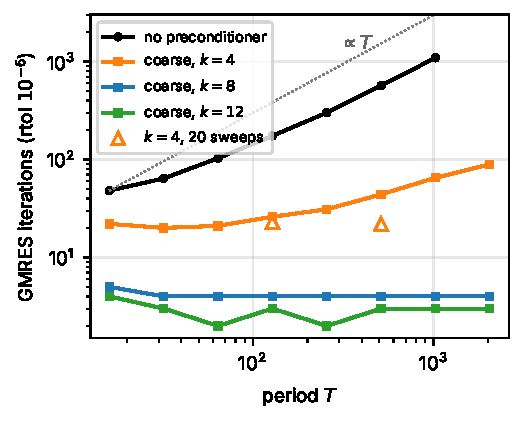
\includegraphics[width=0.55\textwidth]{figs/gmres_trajectory.pdf}
\caption{GMRES iterations versus period, trajectory operators, rtol $10^{-6}$, \texttt{coarse\_sweeps} $= 5$ unless stated.}
\label{fig:traj}
\end{figure}

\begin{table}[t]
\centering
\begin{tabular}{rrrrrr}
\toprule
$N$ & $T$ & no prec. & $k = 4$ & $k = 8$ & $k = 12$\\
\midrule
8 & 16 & 48 & 22 & 5 & 4\\
16 & 32 & 64 & 20 & 4 & 3\\
32 & 64 & 103 & 21 & 4 & 2\\
64 & 128 & 174 & 26 & 4 & 3\\
128 & 256 & 300 & 31 & 4 & 2\\
256 & 512 & 567 & 44 & 4 & 3\\
512 & 1024 & 1089 & 65 & 4 & 3\\
1024 & 2048 & -- & 89 & 4 & 3\\
\midrule
\multicolumn{2}{l}{prediction \eqref{eq:predict}} & & 22 & 3.2 & $<2$\\
\bottomrule
\end{tabular}
\caption{GMRES iterations (Figure~\ref{fig:traj}). All solves were checked with the true residual. The unpreconditioned case was not run at $N = 1024$.}
\label{tab:traj}
\end{table}

Without preconditioner the count grows linearly in $T$ (Table~\ref{tab:traj}, Figure~\ref{fig:traj}). With $k = 8$, at the spectral gap, it is 4 at every period up to $2048$, in agreement with \eqref{eq:predict}: $\log 10^{-6}/\log 0.014 = 3.2$. The cluster radius $0.014$ is also visible in Figure~\ref{fig:spectrum}. With $k = 4$ the prediction is 22, which is met for short orbits, but the count grows for long ones: the gap $\lambda_4 - \lambda_5$ is small and 5 sweeps do not converge the subspace. Table~\ref{tab:sweeps} confirms this: with 20 sweeps $k = 4$ stays at 22--23 up to $T = 512$, and with a single sweep even $k = 8$ degrades.

\begin{table}[t]
\centering
\begin{tabular}{rrrrrrr}
\toprule
 & & \multicolumn{3}{c}{$k = 4$} & \multicolumn{2}{c}{$k = 8$}\\
\cmidrule(lr){3-5}\cmidrule(lr){6-7}
$N$ & $T$ & 1 sweep & 5 sweeps & 20 sweeps & 1 sweep & 5 sweeps\\
\midrule
64 & 128 & 95 & 26 & 23 & 12 & 4\\
256 & 512 & 308 & 44 & 22 & 23 & 4\\
\bottomrule
\end{tabular}
\caption{Effect of the number of subspace sweeps at the first Newton step.}
\label{tab:sweeps}
\end{table}

\subsection{Newton searches on long periodic orbits}

We converged periodic orbits from near recurrences with the hookstep method (\texttt{find\_upo.jl}; periods $52.043$, $53.134$, $76.846$). A long orbit is the $M$-fold repetition of the orbit with $T_0 = 53.134$ ($N_0 = 27$ segments): a genuine periodic orbit of period $MT_0$, with multipliers $\mu_j^M$. We perturb all seeds and the period by a relative $10^{-3}$ and reconverge with \texttt{:ls\_iterative}, GMRES rtol $10^{-3}$ (\texttt{scaling\_upo.jl}). All searches reach residuals between $5\cdot 10^{-13}$ and $3\cdot10^{-11}$ in 3--4 Newton steps.

\begin{table}[t]
\centering
\begin{tabular}{rrrlrlrr}
\toprule
 & & & \multicolumn{2}{c}{$k = 8$} & \multicolumn{2}{c}{no preconditioner} & \\
\cmidrule(lr){4-5}\cmidrule(lr){6-7}
$M$ & $N$ & $T$ & GMRES/step & work & GMRES/step & work & ratio\\
\midrule
1 & 27 & 53.1 & 3, 3, 2 & 2\,025 & 79, 81, 81 & 6\,588 & 3.3\\
2 & 54 & 106.3 & 3, 2, 3 & 4\,050 & 135, 135, 135 & 22\,032 & 5.4\\
4 & 108 & 212.5 & 3, 3, 2 & 8\,100 & 243, 244, 243 & 79\,164 & 9.8\\
8 & 216 & 425.1 & 3, 3, 3 & 16\,416 & 456, 460, 435, 455 & 390\,960 & 23.8\\
\bottomrule
\end{tabular}
\caption{Newton searches on repeated orbits. ``Work'' is the number of segment tangent integrations of the whole search: GMRES products, one initial residual per solve, and for $k = 8$ the coarse space ($k$ per step plus $5k$ at the first step). Nonlinear integrations (residuals, line search, period differences) are the same for both and are not counted. Wall time at $M = 8$ on two cores: 34\,s against 359\,s.}
\label{tab:upo}
\end{table}

\begin{figure}[t]
\centering
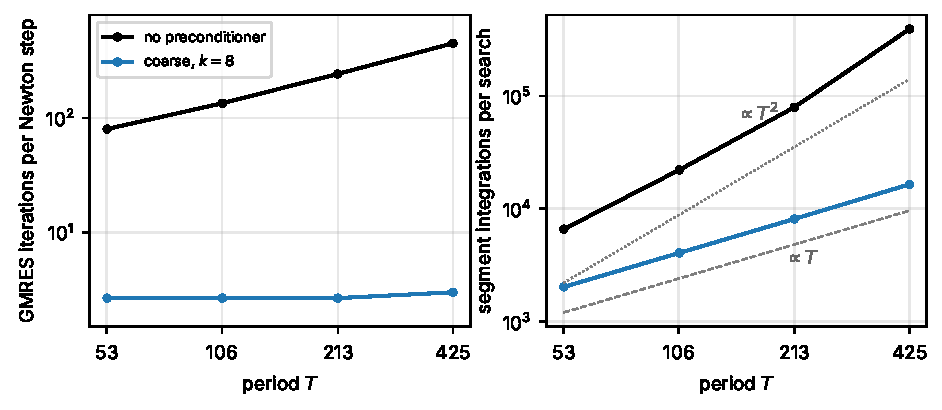
\includegraphics[width=\textwidth]{figs/newton_upo.pdf}
\caption{Newton searches on repeated orbits (Table~\ref{tab:upo}). Left: mean GMRES iterations per Newton step. Right: segment tangent integrations of the whole search, coarse-space cost included.}
\label{fig:upo}
\end{figure}

The total work of a search is proportional to $T$ with the coarse space and to $T^2$ without, so the gain grows linearly with the period (Table~\ref{tab:upo}, Figure~\ref{fig:upo}). At rtol $10^{-3}$ the coarse runs need 2--3 iterations; most of their cost is the coarse space itself (64 of the 76 integrations per segment at $M = 8$), which is the price of making the count independent of $T$.

%======================================================================
\section{Relation to Newton--Picard and to two-grid methods}
%======================================================================

The construction is the multiple-shooting counterpart of the Newton--Picard method of Lust, Roose, Spence and Champneys~\cite{lust1998}. For single shooting, that method splits the state space into the subspace of the dominant Floquet multipliers, computed by subspace iteration with monodromy products, and its complement. It applies Newton to the small projected system and Picard (fixed-point) iteration to the complement, where all multipliers are below a threshold $\rho < 1$. The correspondence is:

\begin{center}
\begin{tabular}{p{0.42\textwidth}p{0.48\textwidth}}
\toprule
Newton--Picard (single shooting) & this preconditioner (multiple shooting)\\
\midrule
dominant Floquet subspace at $x_0$ & covariant subspace $V_i$ at every seed, by the same subspace iteration distributed over the segments\\
Newton on the $p\times p$ projected system & exact Galerkin solve with $E$, size $Nk + N_s$\\
Picard iteration on the complement & $-I$ on the complement. With the Ashtari ordering, Richardson iteration with $M = -I$ is Picard propagation along the segments; GMRES accelerates it\\
\bottomrule
\end{tabular}
\end{center}

Iterated as a stationary method, the preconditioner would be a multiple-shooting Newton--Picard iteration. Using it inside GMRES instead has two advantages: GMRES removes the effect of an imperfect subspace and of weakly contracting directions (Table~\ref{tab:sweeps}), and the Krylov solve keeps the standard Newton--Krylov globalisation. Newton--Picard splittings used as Krylov preconditioners also appear in Potschka, Mommer, Schl\"oder and Bock~\cite{potschka2012} for time-periodic parabolic optimal control, where a two-grid alternative to the eigenspace splitting is proposed as well.

The differences from single-shooting Newton--Picard are where multiple shooting matters:
\begin{itemize}
\item \emph{Stability for long $T$.} The single-shooting projected system $V\tr(\Phi - I)V$ carries the growth $e^{\lambda_1 T}$. Here the coarse problem keeps the multiple-shooting structure and is solved by QR; this is exactly where LU failed at $T = 1024$.
\item \emph{Parallelism.} Subspace iteration, coarse assembly and Krylov products are all per segment, so the wall time of a Newton step does not depend on $T$.
\end{itemize}

The same principle underlies the space-time two-grid preconditioner of the ReSolver notes: one coarse space contains everything the cheap part of the preconditioner (there the diagonal smoother, here $-I$) does not damp. There the coarse space is organised by scale (low sine modes); here it is organised by Floquet direction. Before claiming the multiple-shooting version is new, the literature on Newton--Picard (including Lust's own work) should be checked for an existing multiple-shooting variant.

%======================================================================
\section{Implementation in NKSearch}
%======================================================================

\paragraph{Usage.}
\begin{verbatim}
opts = Options(method=:ls_iterative,  # row_order=:ashtari is the default
               coarse_dim=8,          # k; 0 disables (default)
               coarse_sweeps=5,       # sweeps at the first Newton step
               gmres_rtol=1e-3, gmres_maxiter=100)
search!(G, L, F, z, opts)
\end{verbatim}
The preconditioner needs nothing beyond what NKSearch already uses: the linearised flow $L$ (applied $k$ times per segment and Newton step), the shift $S$ and the derivative operators. The state type must support \texttt{randn!} (for the random initial bases), \texttt{dot}, \texttt{norm} and broadcasting.

\paragraph{Code.}
\begin{itemize}
\item \texttt{src/coarse\_precond.jl}: the type \texttt{CoarsePrecond} (bases $V$, images $P$, sparse $E$ and its QR), subspace iteration, assembly of $E$, $M^{-1}$ and $M$, and the operator $AM^{-1}$ passed to GMRES.
\item \texttt{src/iter\_sol\_cache.jl}: \texttt{IterSolCache} holds the preconditioner (or \texttt{nothing}), updates it at every Newton step after the period derivatives, and dispatches the preconditioned solve.
\item \texttt{src/options.jl}: options \texttt{coarse\_dim}, \texttt{coarse\_sweeps}.
\item \texttt{test/test\_coarse.jl}: with $k = n$ the preconditioner is $A^{-1}$ and GMRES converges in one iteration; $MM^{-1} = I$; searches converge with partial coarse spaces.
\end{itemize}

\paragraph{Line-search driver.} Two problems in \texttt{src/search\_linesearch.jl} were fixed in a separate commit. The first correction was initialised with \texttt{similar(z0) .*= 0.0}, which keeps NaN from uninitialised memory; it is now \texttt{zero(z0)}, as in the hookstep driver. GMRES was warm-started from the previous Newton correction, which after the first step is much larger than the new right-hand side; GMRES then started from a relative residual of order $10^2$--$10^3$. The driver now applies \texttt{opts.gmres\_start} (default: zero), like the hookstep driver.

\paragraph{Limitations.}
\begin{itemize}
\item Only \texttt{:ls\_iterative} with the Ashtari ordering. For the hookstep, the trust-region constraint must be $\|M^{-1}Q_m y\| \le \Delta$ rather than $\|Q_m y\| \le \Delta$; this requires storing $M^{-1}q_j$ in GMRES.jl (flexible-GMRES style) and solving the hookstep subproblem in that norm.
\item Memory $2Nk$ states.
\item $k$ is fixed by the user. An adaptive choice, as in adaptive Newton--Picard, could monitor the Ritz values of the subspace iteration and enlarge $k$ until a gap is found.
\end{itemize}

%======================================================================
\section{Reproducing the results}
%======================================================================

All scripts are in \texttt{docs/notes/coarse\_precond} and need Flows.jl, GMRES.jl and this branch of NKSearch. Run with \texttt{julia -t 2}:
\begin{itemize}
\item \texttt{ks.jl}: the KS model (included by the other scripts).
\item \texttt{lyapunov.jl}: Lyapunov exponents $\to$ \texttt{data/lyapunov.txt}.
\item \texttt{spectrum.jl}: eigenvalues of Figure~\ref{fig:spectrum} $\to$ \texttt{data/spectrum.txt}.
\item \texttt{scaling\_trajectory.jl}: Table~\ref{tab:traj}; environment variables \texttt{NS}, \texttt{KS}, \texttt{SWEEPS} select the runs $\to$ \texttt{data/trajectory\_*.txt}, \texttt{data/sweeps\_*.txt}.
\item \texttt{find\_upo.jl}: periodic orbits from near recurrences $\to$ \texttt{upos/}.
\item \texttt{scaling\_upo.jl upos/T\_53.134.txt}: Table~\ref{tab:upo}; variables \texttt{MS}, \texttt{KS} $\to$ \texttt{data/upo\_newton.txt}.
\item \texttt{python3 make\_figs.py}: the figures, from \texttt{data/}.
\end{itemize}
The file \texttt{data/trajectory\_k0.txt} comes from a run with the earlier LU coarse solve; only its unpreconditioned rows are used.

\begin{thebibliography}{9}
\bibitem{lust1998} K.~Lust, D.~Roose, A.~Spence, A.~R.~Champneys, An adaptive Newton--Picard algorithm with subspace iteration for computing periodic solutions, \emph{SIAM J.\ Sci.\ Comput.} 19(4), 1188--1209, 1998.
\bibitem{potschka2012} A.~Potschka, M.~S.~Mommer, J.~P.~Schl\"oder, H.~G.~Bock, Newton--Picard-based preconditioning for linear-quadratic optimization problems with time-periodic parabolic PDE constraints, \emph{SIAM J.\ Sci.\ Comput.} 34(2), A1214--A1239, 2012.
\bibitem{wright1993} S.~J.~Wright, A collection of problems for which Gaussian elimination with partial pivoting is unstable, \emph{SIAM J.\ Sci.\ Comput.} 14(1), 231--238, 1993.
\end{thebibliography}

\end{document}
